\documentclass[11pt,a4paper]{article}

\usepackage[utf8]{inputenc}
\usepackage[T1]{fontenc}
\usepackage[spanish, provide=*]{babel}
\usepackage{graphicx}
\usepackage[margin=2.5cm]{geometry}
\usepackage{url}

\emergencystretch=2em
\graphicspath{{../figures/}}

\begin{document}

% =====================================================================
% 1. Portada (pagina aparte, sin numerar)
% =====================================================================
\begin{titlepage}
  \centering
  \vspace*{2.5cm}

  {\LARGE\bfseries Regresión Lineal: recolección de datos y modelado de produccion\_toneladas\par}

  \vspace{1.5cm}

  {\large Taller: Semana 4 -- Herramientas de recolección de datos\par}

  \vspace{2.5cm}

  {\large Curso: Machine Learning\par}
  \vspace{0.4cm}
  {\large Autores: Crsitian Alejandro Perdomo Rivas\par}
  \vspace{0.4cm}
  {\large Fecha: 19/09/2026\par}

  \vfill

  {\normalsize Proyecto de regresión lineal con Python (pandas, scikit-learn) sobre datos de
  producción de frutales en el Valle del Cauca.\par}
\end{titlepage}

\setcounter{page}{1}

% =====================================================================
% 2. Resumen ejecutivo
% =====================================================================
\section{Resumen ejecutivo}

Este informe documenta la recolección, limpieza, modelado y evaluación de un modelo de regresión
lineal que estima la variable continua \texttt{produccion\_toneladas} (toneladas de fruta
producidas) a partir de tres predictores: \texttt{año}, \texttt{id\_municipio} y la variable
categórica \texttt{subregion}. Los datos provienen de un conjunto abierto de producción de frutales
en el Valle del Cauca (Colombia) y, para evitar mezclar especies distintas, el análisis se
restringe al cultivo con más registros, el plátano (943 filas tras limpiar). El modelo, ajustado
con \texttt{LinearRegression} de scikit-learn sobre una partición 80/20 con semilla 42, obtiene en
test $R^2 = 0.1909$ y $\mathrm{RMSE} = 8249.39$ toneladas. La conclusión principal es que el
modelo explica alrededor del 19\% de la varianza: la relación lineal de los predictores disponibles
con la producción es débil y el objetivo está fuertemente sesgado, por lo que el modelo sirve como
línea base más que como predictor preciso.

% =====================================================================
% 3. Método de recolección
% =====================================================================
\section{Método de recolección}

\subsection{Fuente y tipo}

Los datos proceden de un conjunto de datos abiertos (\emph{open data}) con registros de producción
de frutales en el Valle del Cauca (Colombia). El archivo fuente es un CSV con campos delimitados por
comas y entrecomillados. La tabla~\ref{tab:trazabilidad} resume su trazabilidad.

\begin{table}[htbp]
  \centering
  \caption{Trazabilidad del conjunto de datos original.}
  \label{tab:trazabilidad}
  \begin{tabular}{lp{11.5cm}}
    \hline
    Campo & Valor \\
    \hline
    Fuente & Registros de producción de frutales en el Valle del Cauca (Colombia) \\
    URL & \url{https://www.datos.gov.co/browse?q=venta+&sortBy=relevance&pageSize=20} \\
    Fecha de obtención & 2026-09-19 \\
    Formato & CSV (campos entre comillas; decimal con coma) \\
    Filas & 9992 \\
    Columnas & 8 \\
    \hline
  \end{tabular}
\end{table}

\subsection{Pasos de recolección}

Los pasos seguidos en el \emph{notebook} \texttt{01\_recoleccion.ipynb} fueron:

\begin{enumerate}
  \item Se identificó el archivo fuente en \texttt{./files/}.
  \item Se copió, sin modificar, a \texttt{data/raw/} con \texttt{shutil.copy2}.
  \item Se leyó con \texttt{pandas} usando separador por comas y comillas (\texttt{sep=','}).
  \item Se revisó la estructura: nombres de columna, forma del dataset y primeras filas.
  \item Se aplicaron criterios de calidad (nulos, duplicados, tipos y rangos).
\end{enumerate}

\subsection{Criterios de calidad revisados}

Sobre el archivo original de 9992 filas y 8 columnas se verificaron los siguientes criterios:

\begin{itemize}
  \item \textbf{Nulos:} 0 valores nulos en todas las columnas.
  \item \textbf{Duplicados:} 39 filas duplicadas exactas (se eliminan en la limpieza).
  \item \textbf{Tipos de dato:} al leer, \texttt{año}, \texttt{Id\_municipio} e \texttt{Id\_cultivo}
        se interpretan como enteros; \texttt{Produccion\_toneladas} queda como texto y debe
        convertirse a número.
  \item \textbf{Rangos razonables:} el año va de 2000 a 2022; la producción usa formato español
        (punto como separador de miles y coma decimal); hay 202 registros con producción igual a
        cero y ninguno negativo; \texttt{subregion} tiene 4 categorías, \texttt{ciclo} 3,
        \texttt{cultivo} 38 y \texttt{municipio} 42.
\end{itemize}

El dataset cubre 38 cultivos y 42 municipios. Para este taller se seleccionó únicamente el cultivo
\textbf{plátano}, por ser el de mayor número de registros (943 filas). Tras el filtro, las columnas
\texttt{cultivo}, \texttt{id\_cultivo} y \texttt{ciclo} quedan constantes (para el plátano el ciclo
es siempre \emph{Anual}) y se descartan junto con \texttt{municipio} (texto duplicado del
identificador). El dataset limpio final tiene 943 filas y 4 columnas y se guarda en
\texttt{data/processed/frutales\_limpias.csv}.

% =====================================================================
% 4. Análisis exploratorio (EDA)
% =====================================================================
\section{Análisis exploratorio}

\subsection{Diccionario de variables}

La tabla~\ref{tab:diccionario} describe las variables del dataset limpio.

\begin{table}[htbp]
  \centering
  \caption{Diccionario de variables del dataset limpio.}
  \label{tab:diccionario}
  \small
  \begin{tabular}{lp{6cm}ll}
    \hline
    Variable & Descripción & Tipo & Rol \\
    \hline
    produccion\_toneladas & Toneladas de fruta producidas & numérica (float) & Objetivo \\
    año & Año del registro (2000--2022) & numérica (int) & Predictor \\
    id\_municipio & Identificador numérico del municipio & numérica (int) & Predictor \\
    subregion & Región geográfica (Centro, Norte, Pacifico, Sur) & categórica & Predictor \\
    \hline
  \end{tabular}
\end{table}

\subsection{Estadísticos descriptivos}

La tabla~\ref{tab:descriptivos} resume las variables numéricas. La variable categórica
\texttt{subregion} presenta 4 categorías, siendo \emph{Norte} la más frecuente con 368 registros.

\begin{table}[htbp]
  \centering
  \caption{Estadísticos descriptivos de las variables numéricas (n = 943).}
  \label{tab:descriptivos}
  \footnotesize
  \setlength{\tabcolsep}{4pt}
  \begin{tabular}{lrrrrrrr}
    \hline
    Variable & Media & Desv. & Mín. & P25 & Mediana & P75 & Máx. \\
    \hline
    produccion\_toneladas & 5346.90 & 9997.69 & 33 & 775 & 1978 & 4771 & 105000 \\
    año & 2010.88 & 6.65 & 2000 & 2005 & 2011 & 2017 & 2022 \\
    id\_municipio & 76414 & 300 & 76001 & 76126 & 76364 & 76670 & 76895 \\
    \hline
  \end{tabular}
\end{table}

La distribución de la producción (Figura~\ref{fig:hist_objetivo}) es fuertemente asimétrica hacia
la derecha: la mediana es 1978 t mientras que el máximo alcanza 105\,000 t. Esto implica que unos
pocos valores extremos dominan la escala y anticipan que los residuos del modelo no serán
simétricos.

\begin{figure}[htbp]
  \centering
  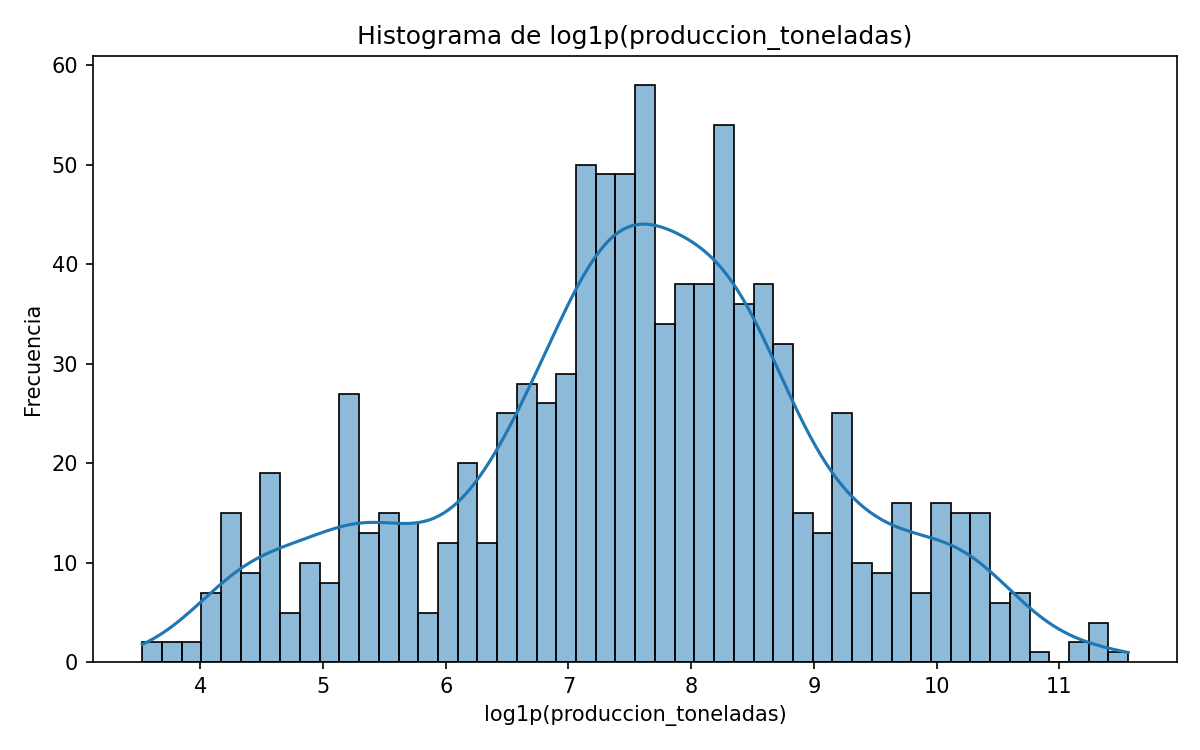
\includegraphics[width=0.8\textwidth]{histograma_objetivo.png}
  \caption{Distribución de la variable objetivo (transformación log1p para visualizar el sesgo).}
  \label{fig:hist_objetivo}
\end{figure}

\subsection{Correlación}

La matriz de correlación de las variables numéricas (Figura~\ref{fig:correlacion}) muestra
correlaciones débiles entre todas las parejas. La más alta con el objetivo la presenta
\texttt{año}, con $r = 0.171$ (valor reportado por el \emph{notebook} 04); el resto de correlaciones
son aún menores. Esto sugiere que la relación lineal entre los predictores disponibles y la
producción es limitada.

\begin{figure}[htbp]
  \centering
  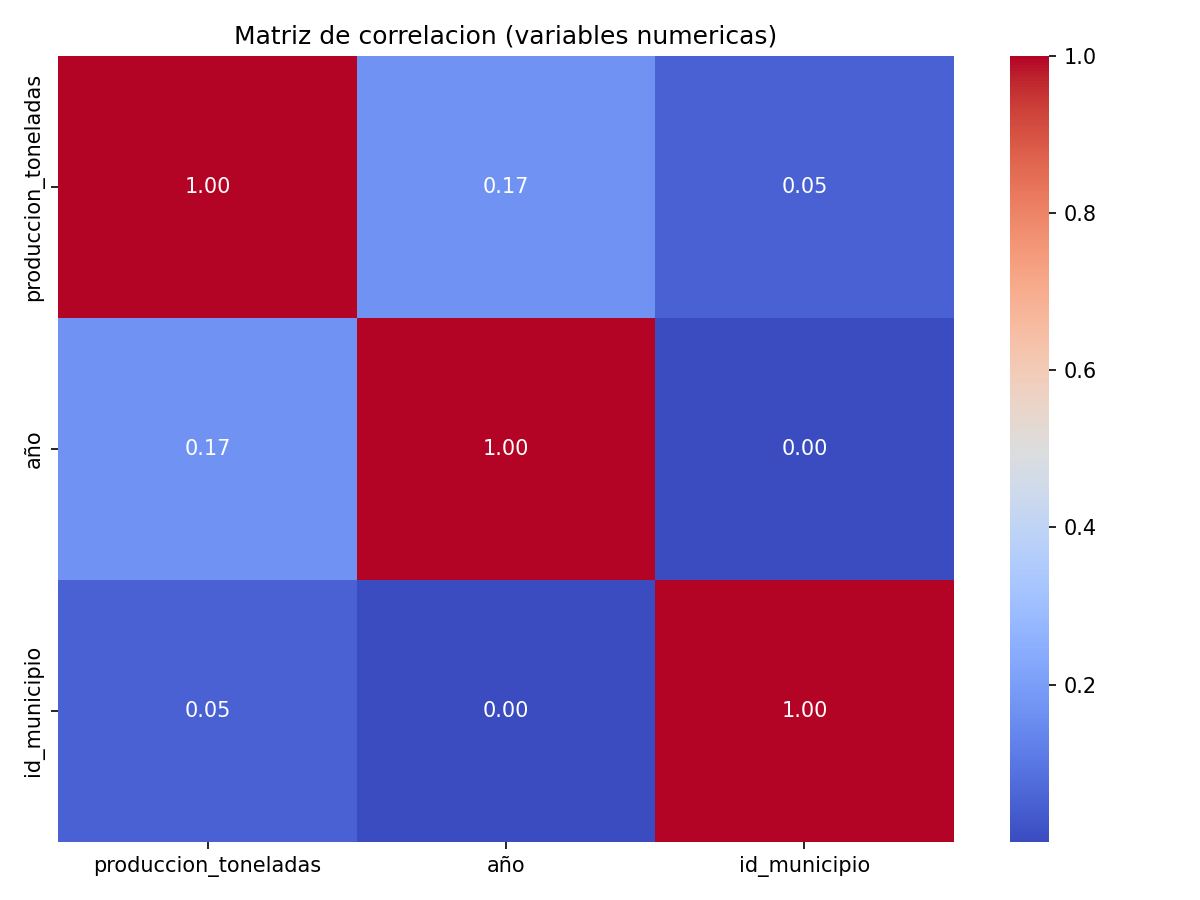
\includegraphics[width=0.8\textwidth]{matriz_correlacion.png}
  \caption{Matriz de correlación de las variables numéricas.}
  \label{fig:correlacion}
\end{figure}

\subsection{Relación de cada predictor con el objetivo}

La Figura~\ref{fig:scatter} muestra la relación de cada predictor con la producción: las variables
numéricas (\texttt{año} e \texttt{id\_municipio}) como diagramas de dispersión y la categórica
(\texttt{subregion}) como diagrama de cajas. No se observa una tendencia lineal clara en ningún
caso; las medianas de producción son parecidas entre subregiones.

\begin{figure}[htbp]
  \centering
  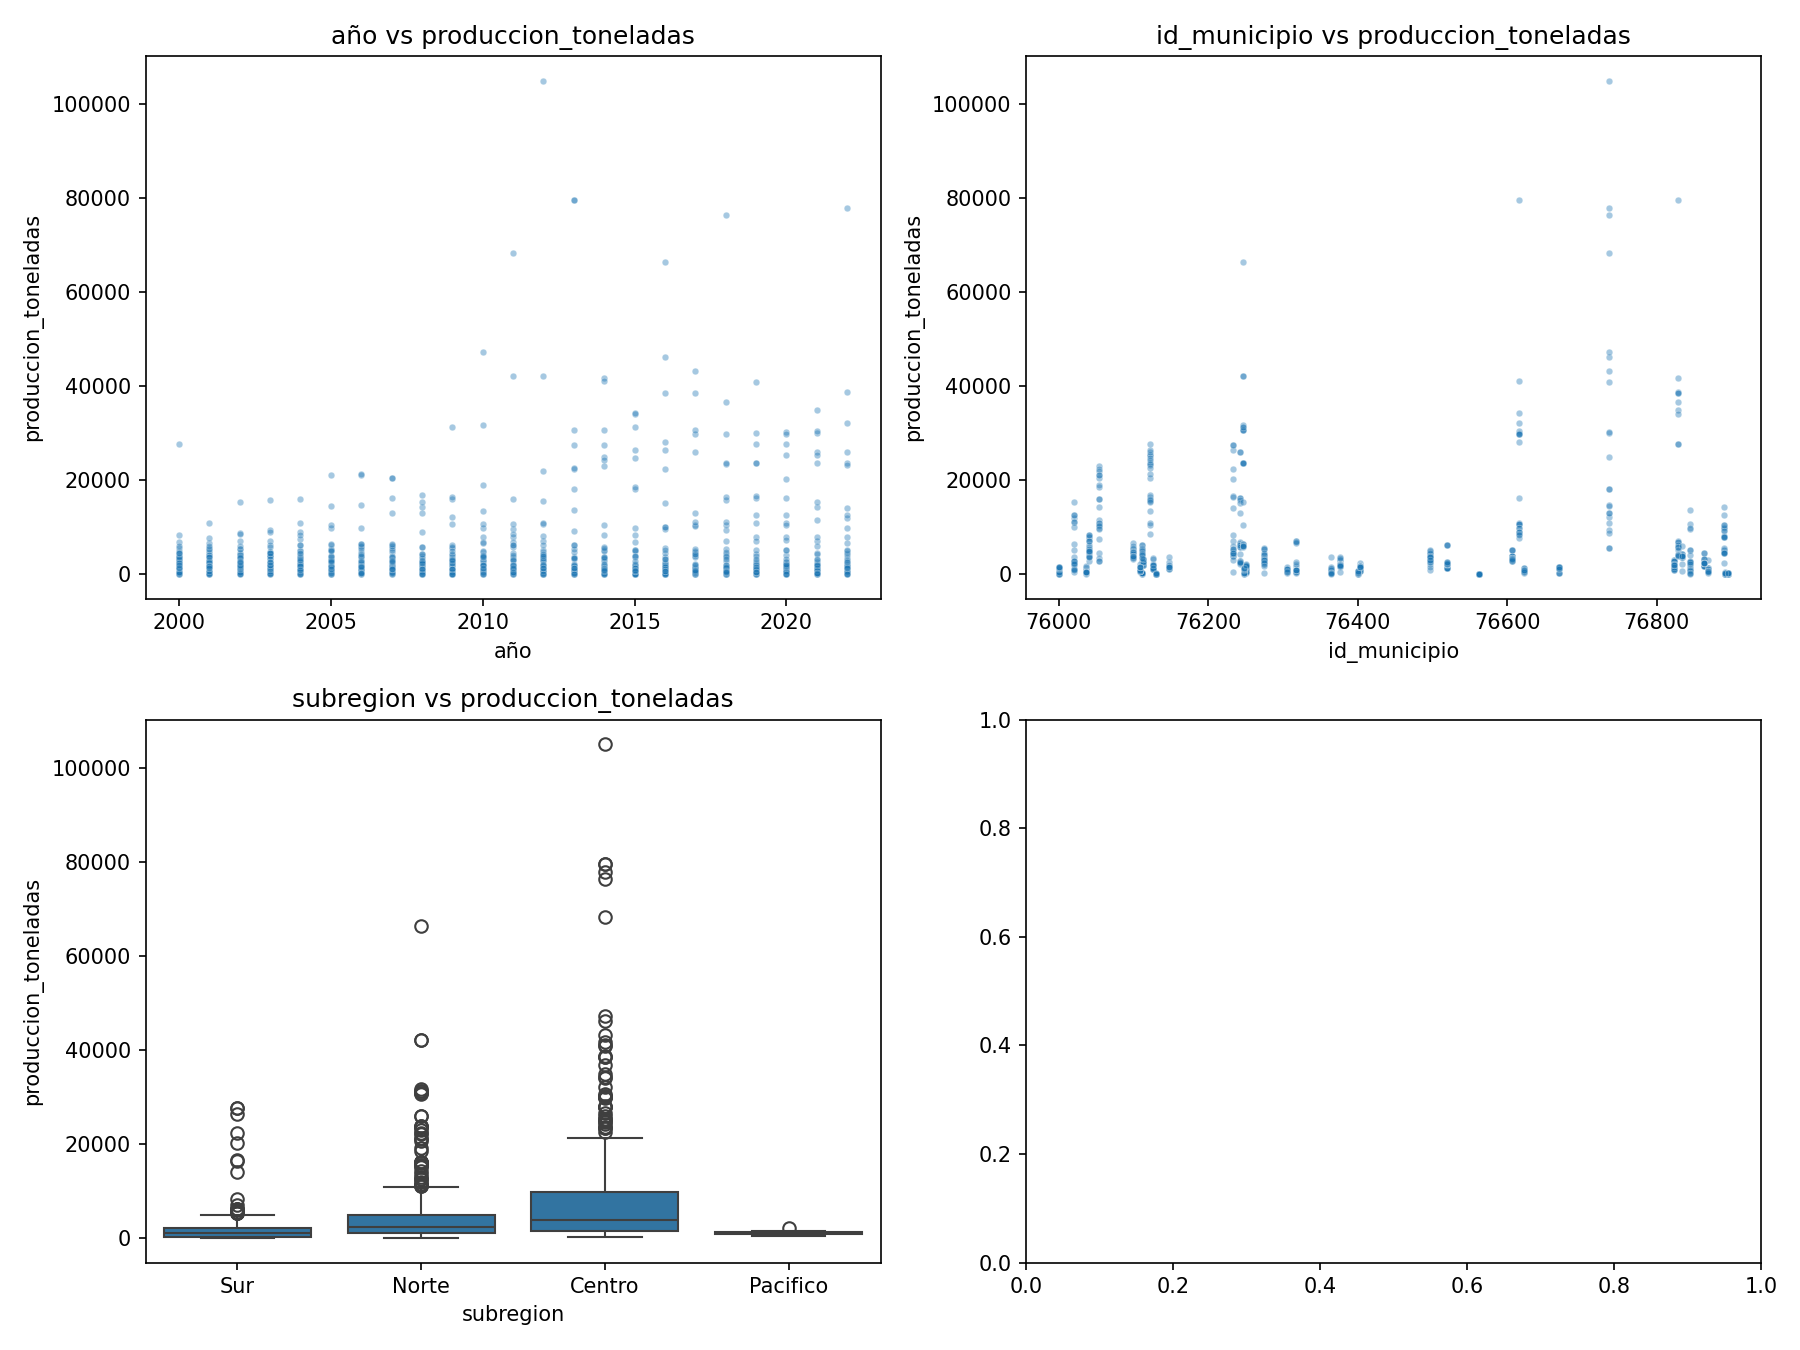
\includegraphics[width=0.95\textwidth]{scatter_predictores_objetivo.png}
  \caption{Relación de cada predictor con la variable objetivo.}
  \label{fig:scatter}
\end{figure}

% =====================================================================
% 5. Modelo
% =====================================================================
\section{Modelo}

\subsection{Configuración}

El modelo se ajustó en el \emph{notebook} \texttt{03\_modelo.ipynb} con la siguiente configuración:

\begin{itemize}
  \item \textbf{Partición:} \texttt{train\_test\_split} con 80\% de entrenamiento (754 filas) y
        20\% de prueba (189 filas); \texttt{test\_size=0.2} y \texttt{random\_state=42}.
  \item \textbf{Tratamiento de categóricas:} la variable \texttt{subregion} (4 categorías) se
        codificó con \texttt{pd.get\_dummies(drop\_first=}\allowbreak\texttt{True)}, generando 3 variables binarias
        (\texttt{subregion\_Norte}, \texttt{subregion\_Pacifico}, \texttt{subregion\_Sur}) y dejando
        \texttt{Centro} como categoría base.
  \item \textbf{Variables usadas:} \texttt{año}, \texttt{id\_municipio} y los dummies de
        \texttt{subregion}. Se justifican porque describen cuándo, dónde y en qué subregión se
        produce; el cultivo se fija a plátano para eliminar el efecto de la especie.
  \item \textbf{Algoritmo:} \texttt{LinearRegression} de scikit-learn.
\end{itemize}

\subsection{Coeficientes e intercepto}

La tabla~\ref{tab:coeficientes} presenta los coeficientes estimados. El intercepto no tiene una
interpretación práctica directa (es el valor predicho cuando todos los predictores valen cero, lo
que obliga a extrapolar la recta de la variable \texttt{año} hasta el año 0). Los coeficientes con
mayor magnitud son los de \texttt{subregion}: respecto a la base \texttt{Centro}, la subregión
\texttt{Pacifico} se asocia con $-7881.80$ t y \texttt{Sur} con $-7111.30$ t, mientras que
\texttt{Norte} aporta $-4302.00$ t. La variable \texttt{año} aporta $+240.59$ t por cada año
adicional, y \texttt{id\_municipio} tiene un efecto despreciable ($+0.45$ t por unidad de código).

\begin{table}[htbp]
  \centering
  \caption{Coeficientes e intercepto del modelo de regresión lineal.}
  \label{tab:coeficientes}
  \begin{tabular}{lr}
    \hline
    Variable & Coeficiente \\
    \hline
    Intercepto ($b_0$) & -509200.34 \\
    año & 240.59 \\
    id\_municipio & 0.45 \\
    subregion\_Norte & -4302.00 \\
    subregion\_Pacifico & -7881.80 \\
    subregion\_Sur & -7111.30 \\
    \hline
  \end{tabular}
\end{table}

\subsection{Validación de supuestos}

\subsubsection{Linealidad}

La linealidad se revisa con el gráfico de residuos frente a predicciones (Figura~\ref{fig:resid_pred}).
Los residuos no muestran un patrón curvo claro, sino una nube alrededor de cero dominada por unos
pocos puntos extremos (grandes residuos negativos para las producciones altas, que el modelo
subestima). El supuesto de linealidad se cumple \textbf{parcialmente}.

\begin{figure}[htbp]
  \centering
  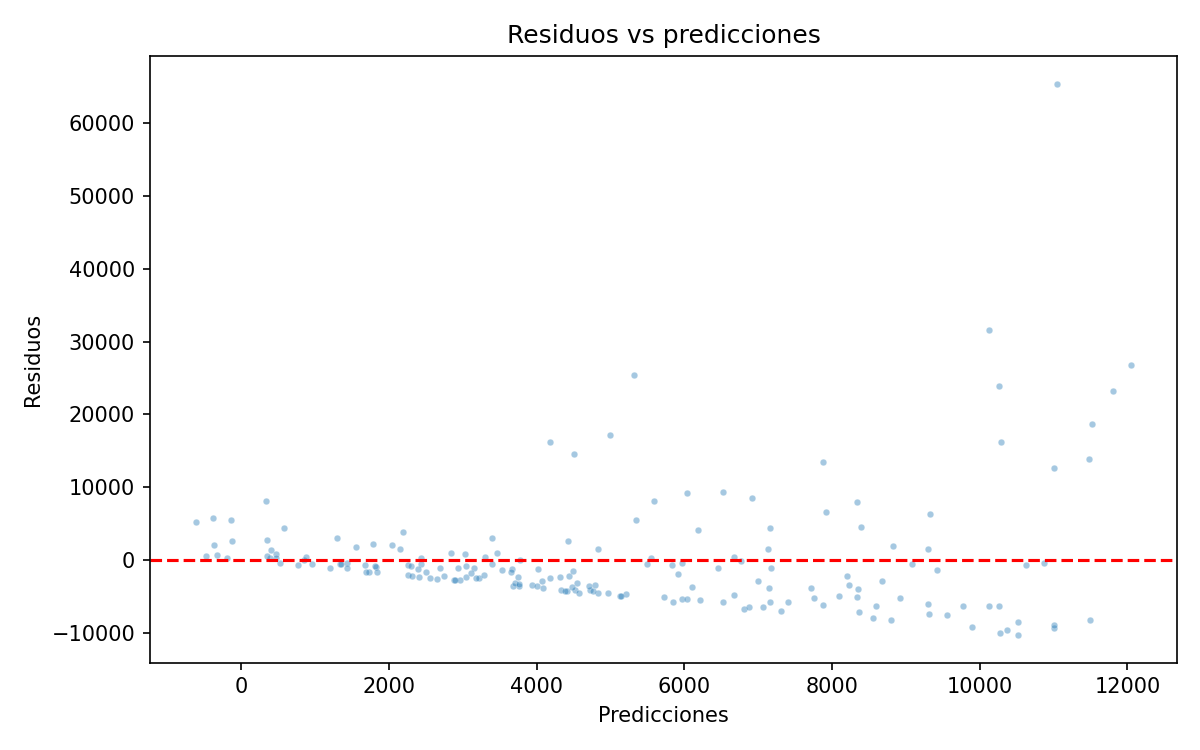
\includegraphics[width=0.8\textwidth]{residuos_vs_predicciones.png}
  \caption{Residuos frente a predicciones (linealidad y homocedasticidad).}
  \label{fig:resid_pred}
\end{figure}

\subsubsection{Homocedasticidad}

En el mismo gráfico (Figura~\ref{fig:resid_pred}) se observa que la dispersión vertical no es
constante: los residuos extremos concentran la mayor parte de la varianza y generan una forma de
embudo. Además, al ser los predictores débiles, las predicciones se agrupan en un rango pequeño. El
supuesto de homocedasticidad \textbf{no se cumple} (heterocedasticidad).

\subsubsection{Distribución de los residuos}

El histograma (Figura~\ref{fig:hist_resid}, con transformación signo $\cdot \log(1+|r|)$ para
comprimir los extremos) y el gráfico Q--Q (Figura~\ref{fig:qq}) muestran que los residuos tienen
colas pesadas y se desvían de la normal en los extremos. El supuesto de normalidad \textbf{no se
cumple}, algo esperable dado el sesgo del objetivo.

\begin{figure}[htbp]
  \centering
  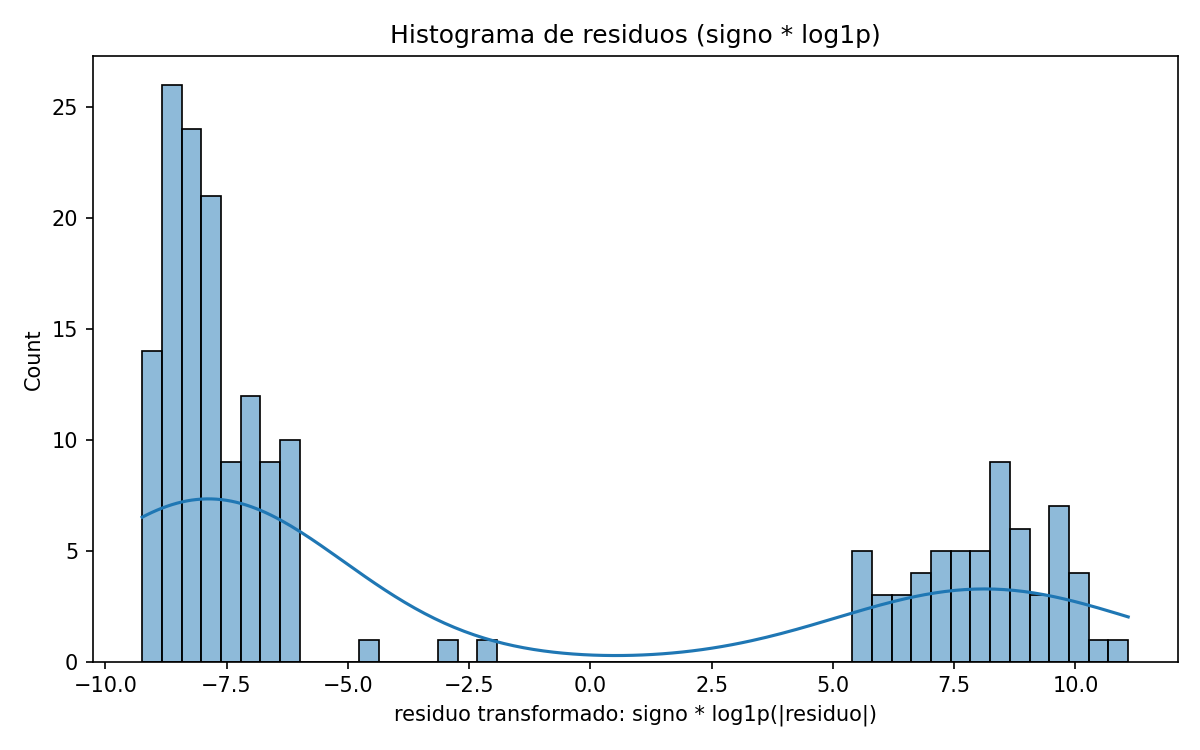
\includegraphics[width=0.8\textwidth]{histograma_residuos.png}
  \caption{Histograma de los residuos (transformación signo $\cdot$ log1p).}
  \label{fig:hist_resid}
\end{figure}

\begin{figure}[htbp]
  \centering
  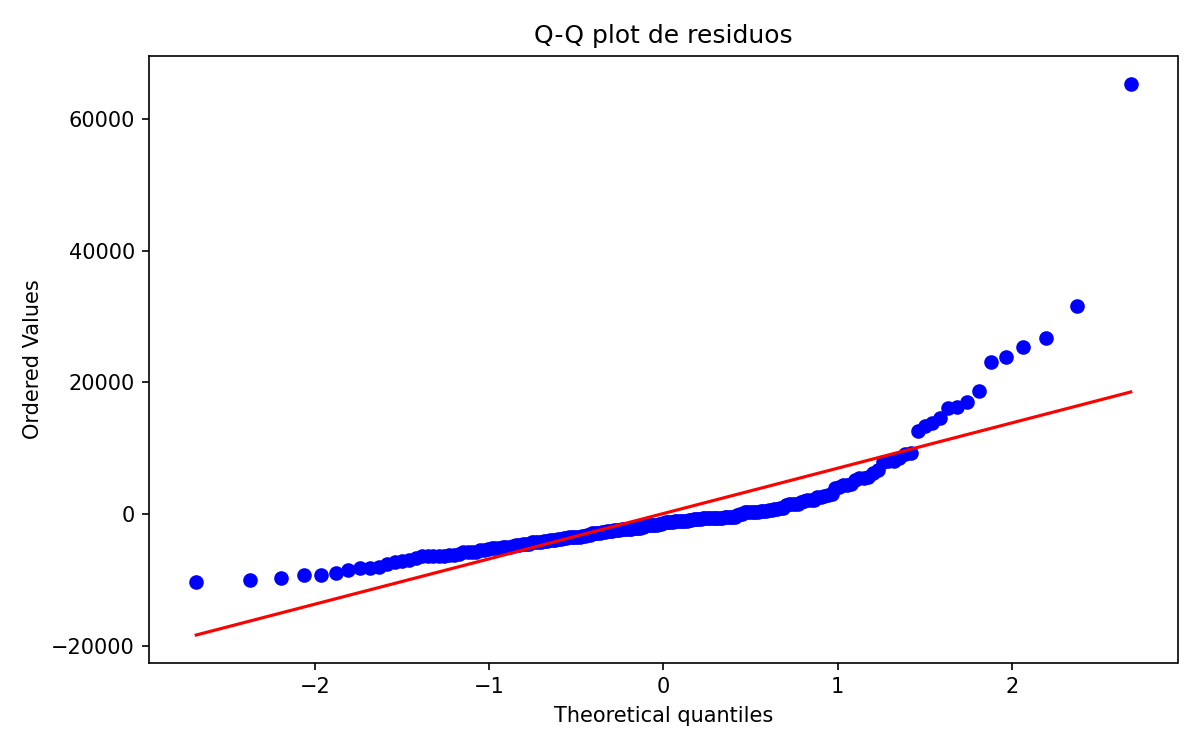
\includegraphics[width=0.8\textwidth]{qq_residuos.png}
  \caption{Gráfico Q--Q de los residuos.}
  \label{fig:qq}
\end{figure}

% =====================================================================
% 6. Evaluación
% =====================================================================
\section{Evaluación}

La tabla~\ref{tab:metricas} resume las métricas calculadas sobre el conjunto de prueba
(189 observaciones).

\begin{table}[htbp]
  \centering
  \caption{Métricas de error sobre el conjunto de prueba.}
  \label{tab:metricas}
  \begin{tabular}{lr}
    \hline
    Métrica & Valor \\
    \hline
    MAE & 4838.09 \\
    MSE & $6.81\times 10^{7}$ \\
    RMSE & 8249.39 \\
    $R^2$ & 0.1909 \\
    \hline
  \end{tabular}
\end{table}

El MAE y el RMSE están en las mismas unidades que el objetivo (toneladas). Un RMSE de 8249.39 t es
grande frente a la mediana de la producción (1978 t), lo que refleja que el error está inflado por
los valores extremos. El $R^2 = 0.1909$ indica que el modelo explica alrededor del 19\% de la
varianza de la producción en test, un poder predictivo modesto pero coherente con las correlaciones
débiles observadas en el EDA.

La Figura~\ref{fig:real_pred} compara valores reales y predichos frente a la recta $y = x$; los
puntos se alejan de la diagonal, sobre todo en los valores altos. La Figura~\ref{fig:regresion_top}
muestra la recta de regresión del predictor numérico más correlacionado (\texttt{año}, $r = 0.171$),
con una pendiente positiva débil. Finalmente, la Figura~\ref{fig:eval_resid} confirma el patrón de
residuos ya comentado.

\begin{figure}[htbp]
  \centering
  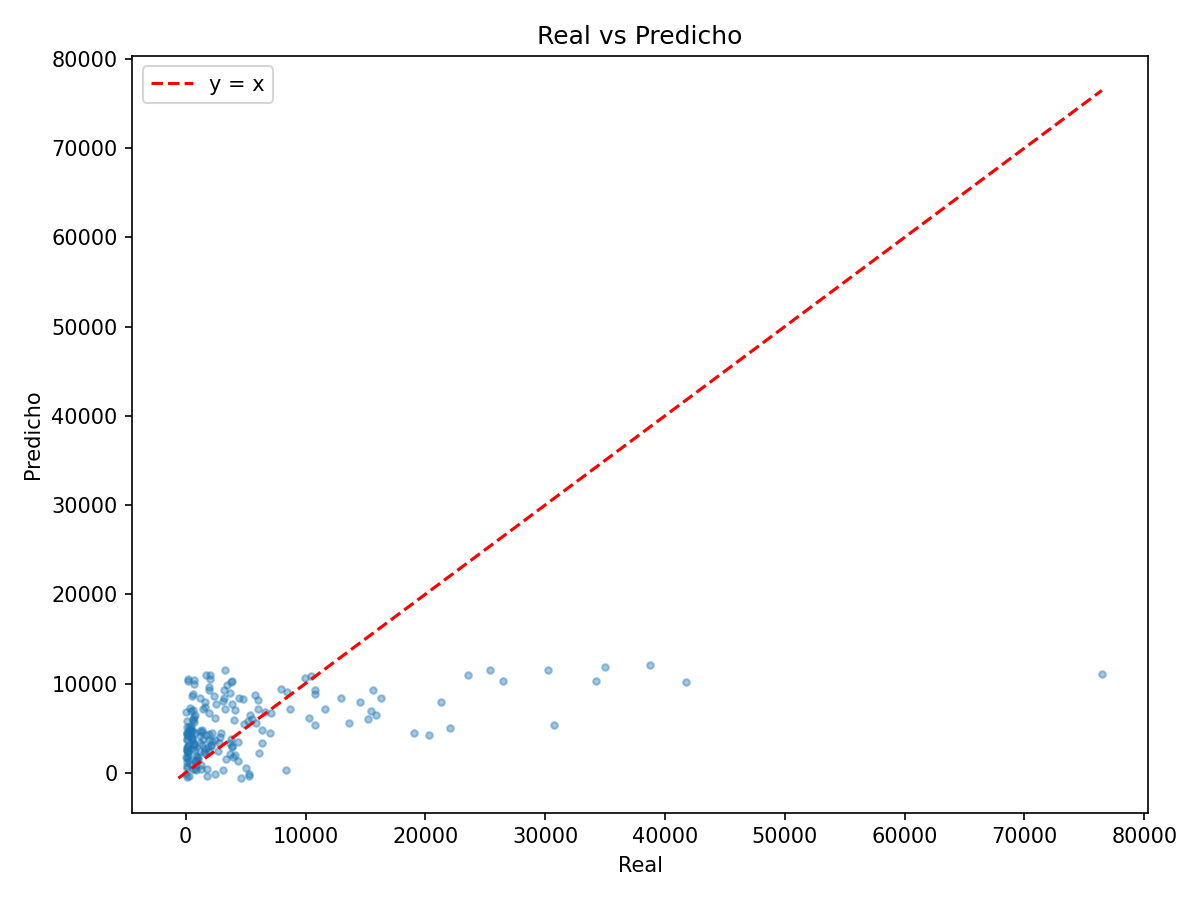
\includegraphics[width=0.8\textwidth]{real_vs_predicho.png}
  \caption{Valores reales frente a predichos, con la recta $y = x$.}
  \label{fig:real_pred}
\end{figure}

\begin{figure}[htbp]
  \centering
  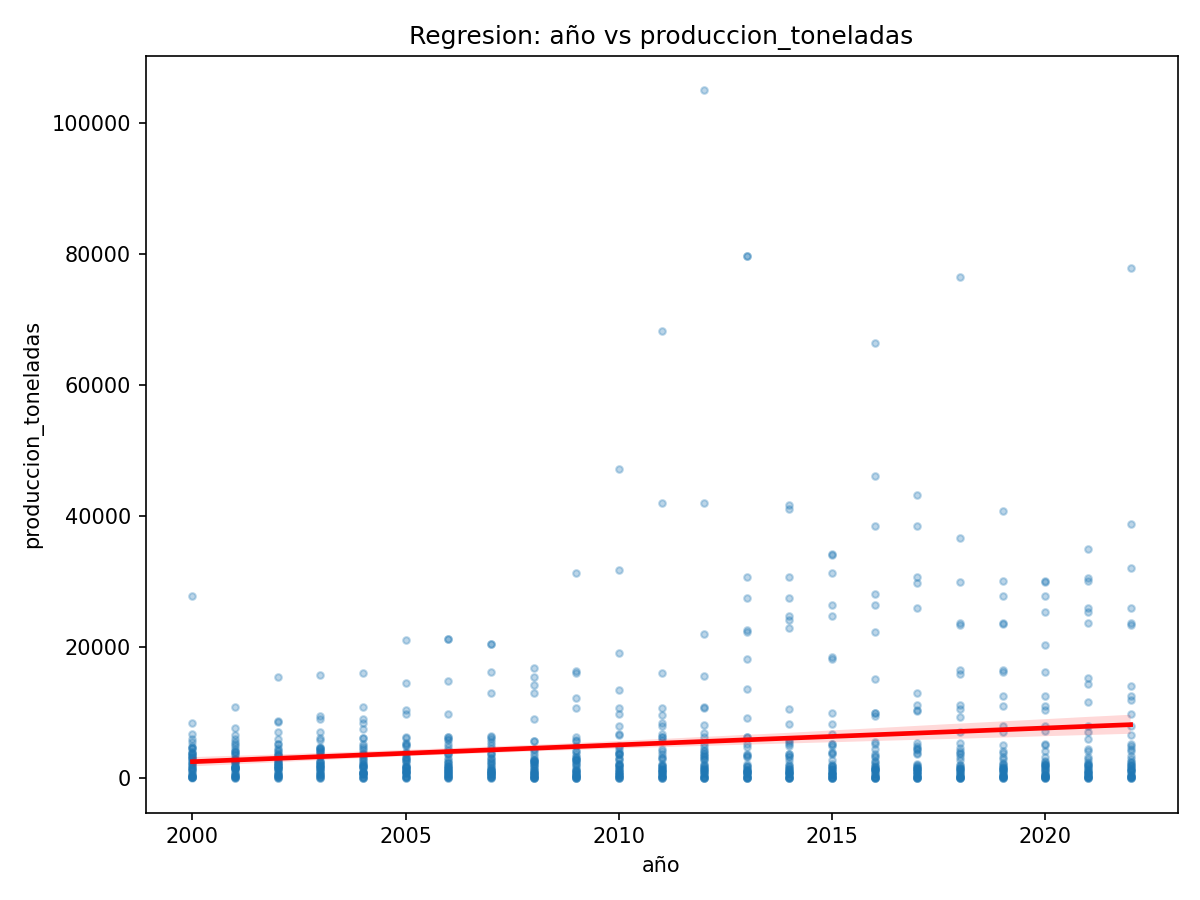
\includegraphics[width=0.8\textwidth]{regresion_predictor_top.png}
  \caption{Dispersión y recta de regresión del predictor más correlacionado (año).}
  \label{fig:regresion_top}
\end{figure}

\begin{figure}[htbp]
  \centering
  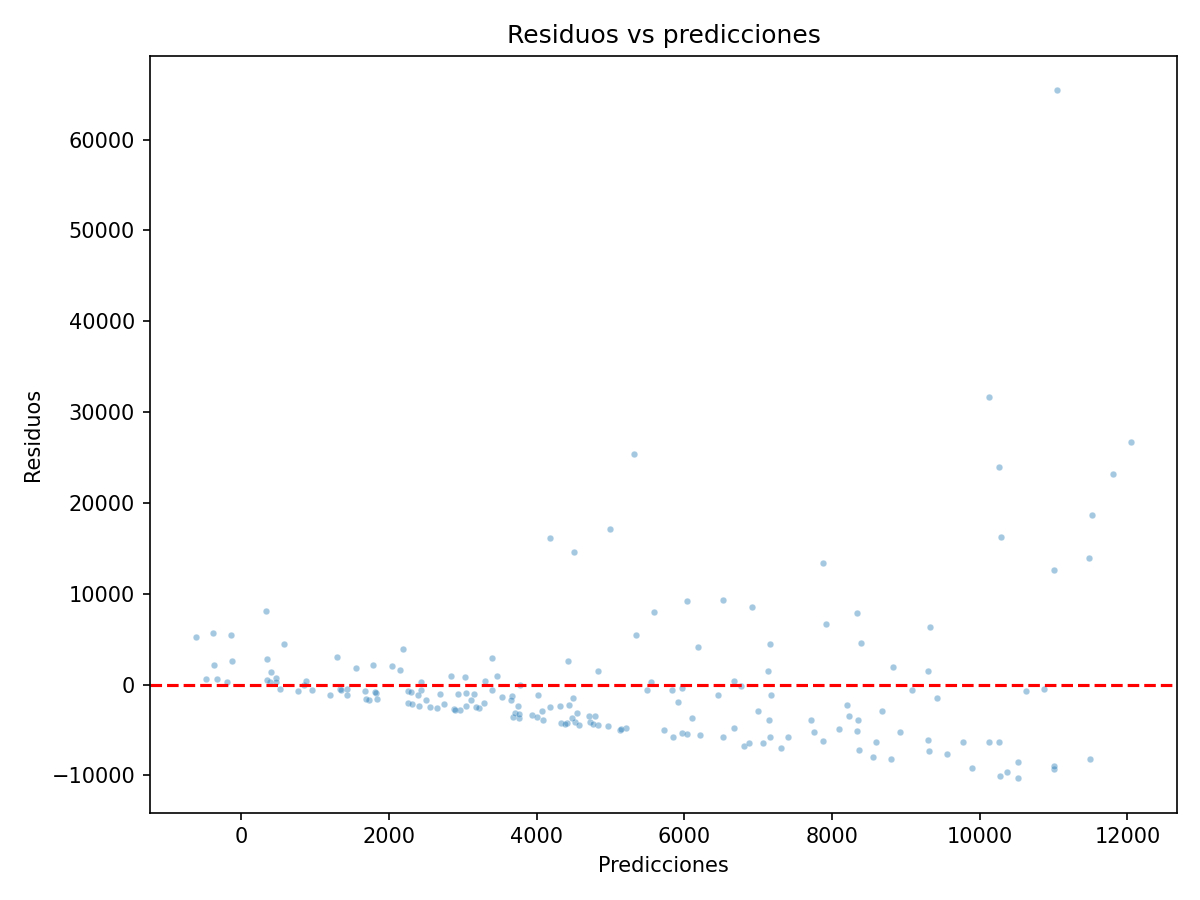
\includegraphics[width=0.8\textwidth]{evaluacion_residuos.png}
  \caption{Residuos frente a predicciones en el conjunto de prueba.}
  \label{fig:eval_resid}
\end{figure}

% =====================================================================
% 7. Conclusiones y trabajo futuro
% =====================================================================
\section{Conclusiones y trabajo futuro}

\subsection{Hallazgos}

El modelo lineal explica el 19.09\% de la varianza de la producción en test, con un RMSE de
8249.39 t. La relación entre los predictores y el objetivo es débil, y la producción está dominada
por unos pocos valores muy grandes que el modelo no logra capturar.

\subsection{Variables más relevantes}

Por magnitud de coeficiente, las variables más relevantes son las categorías de \texttt{subregion}
(en particular \texttt{Pacifico}, $-7881.80$ t respecto a \texttt{Centro}), seguidas de
\texttt{año} ($+240.59$ t por año). \texttt{id\_municipio} tiene un efecto despreciable.

\subsection{Sesgos y limitaciones}

\begin{itemize}
  \item \texttt{id\_municipio} se trató como variable numérica, aunque es un código categórico.
  \item El análisis se limita a un solo cultivo (plátano), por lo que no generaliza a otros frutales.
  \item La producción está muy sesgada a la derecha (mediana 1978 t frente a un máximo de
        105\,000 t), lo que viola los supuestos de homocedasticidad y normalidad.
  \item El modelo solo dispone de tres predictores; variables como el cultivo (38 categorías) se
        descartaron por granularidad, perdiendo información.
\end{itemize}

\subsection{Mejoras futuras}

\begin{itemize}
  \item Modelar el logaritmo de la producción (transformación log1p) para reducir el sesgo y
        estabilizar la varianza.
  \item Incorporar el cultivo como variable categórica (con codificación adecuada) en lugar de
        filtrar a un único cultivo.
  \item Probar modelos no lineales (por ejemplo, árboles de decisión).
  \item Documentar la URL de la fuente y repetir el análisis por subregión.
\end{itemize}

% =====================================================================
% 8. Repositorio GitHub
% =====================================================================
\section{Repositorio GitHub}

El repositorio del proyecto se encuentra en el siguiente enlace:

\begin{center}
\url{https://github.com/CAlejandroPerdomo/UDEC-Regresion-Lineal}
\end{center}

La estructura de carpetas es la siguiente:

\begin{verbatim}
.
|-- data/
|   |-- raw/                          # archivo original, sin modificar
|   `-- processed/                    # dataset limpio (frutales_limpias.csv)
|-- notebooks/
|   |-- 01_recoleccion.ipynb
|   |-- 02_eda.ipynb
|   |-- 03_modelo.ipynb
|   `-- 04_evaluacion.ipynb
|-- figures/                          # graficos en PNG
|-- requirements.txt
`-- README.md
\end{verbatim}

\end{document}
